


  %\system, illustrated in Figure \ref{fig:system}, is a processor architecture which aims at providing secure code execution by means of \puf-based authentication of cache lines. The central idea behind \system~is a \puf-Tag (\ptag) Memory, which runs in parallel with the system main memory (Figure \ref{fig:system}). Each entry in the \ptag~Memory stores an authentication code of a cache line generated by a \puf-based device located on-chip.
  
%   \begin{figure*}[!ht]
% 	\centering
% 	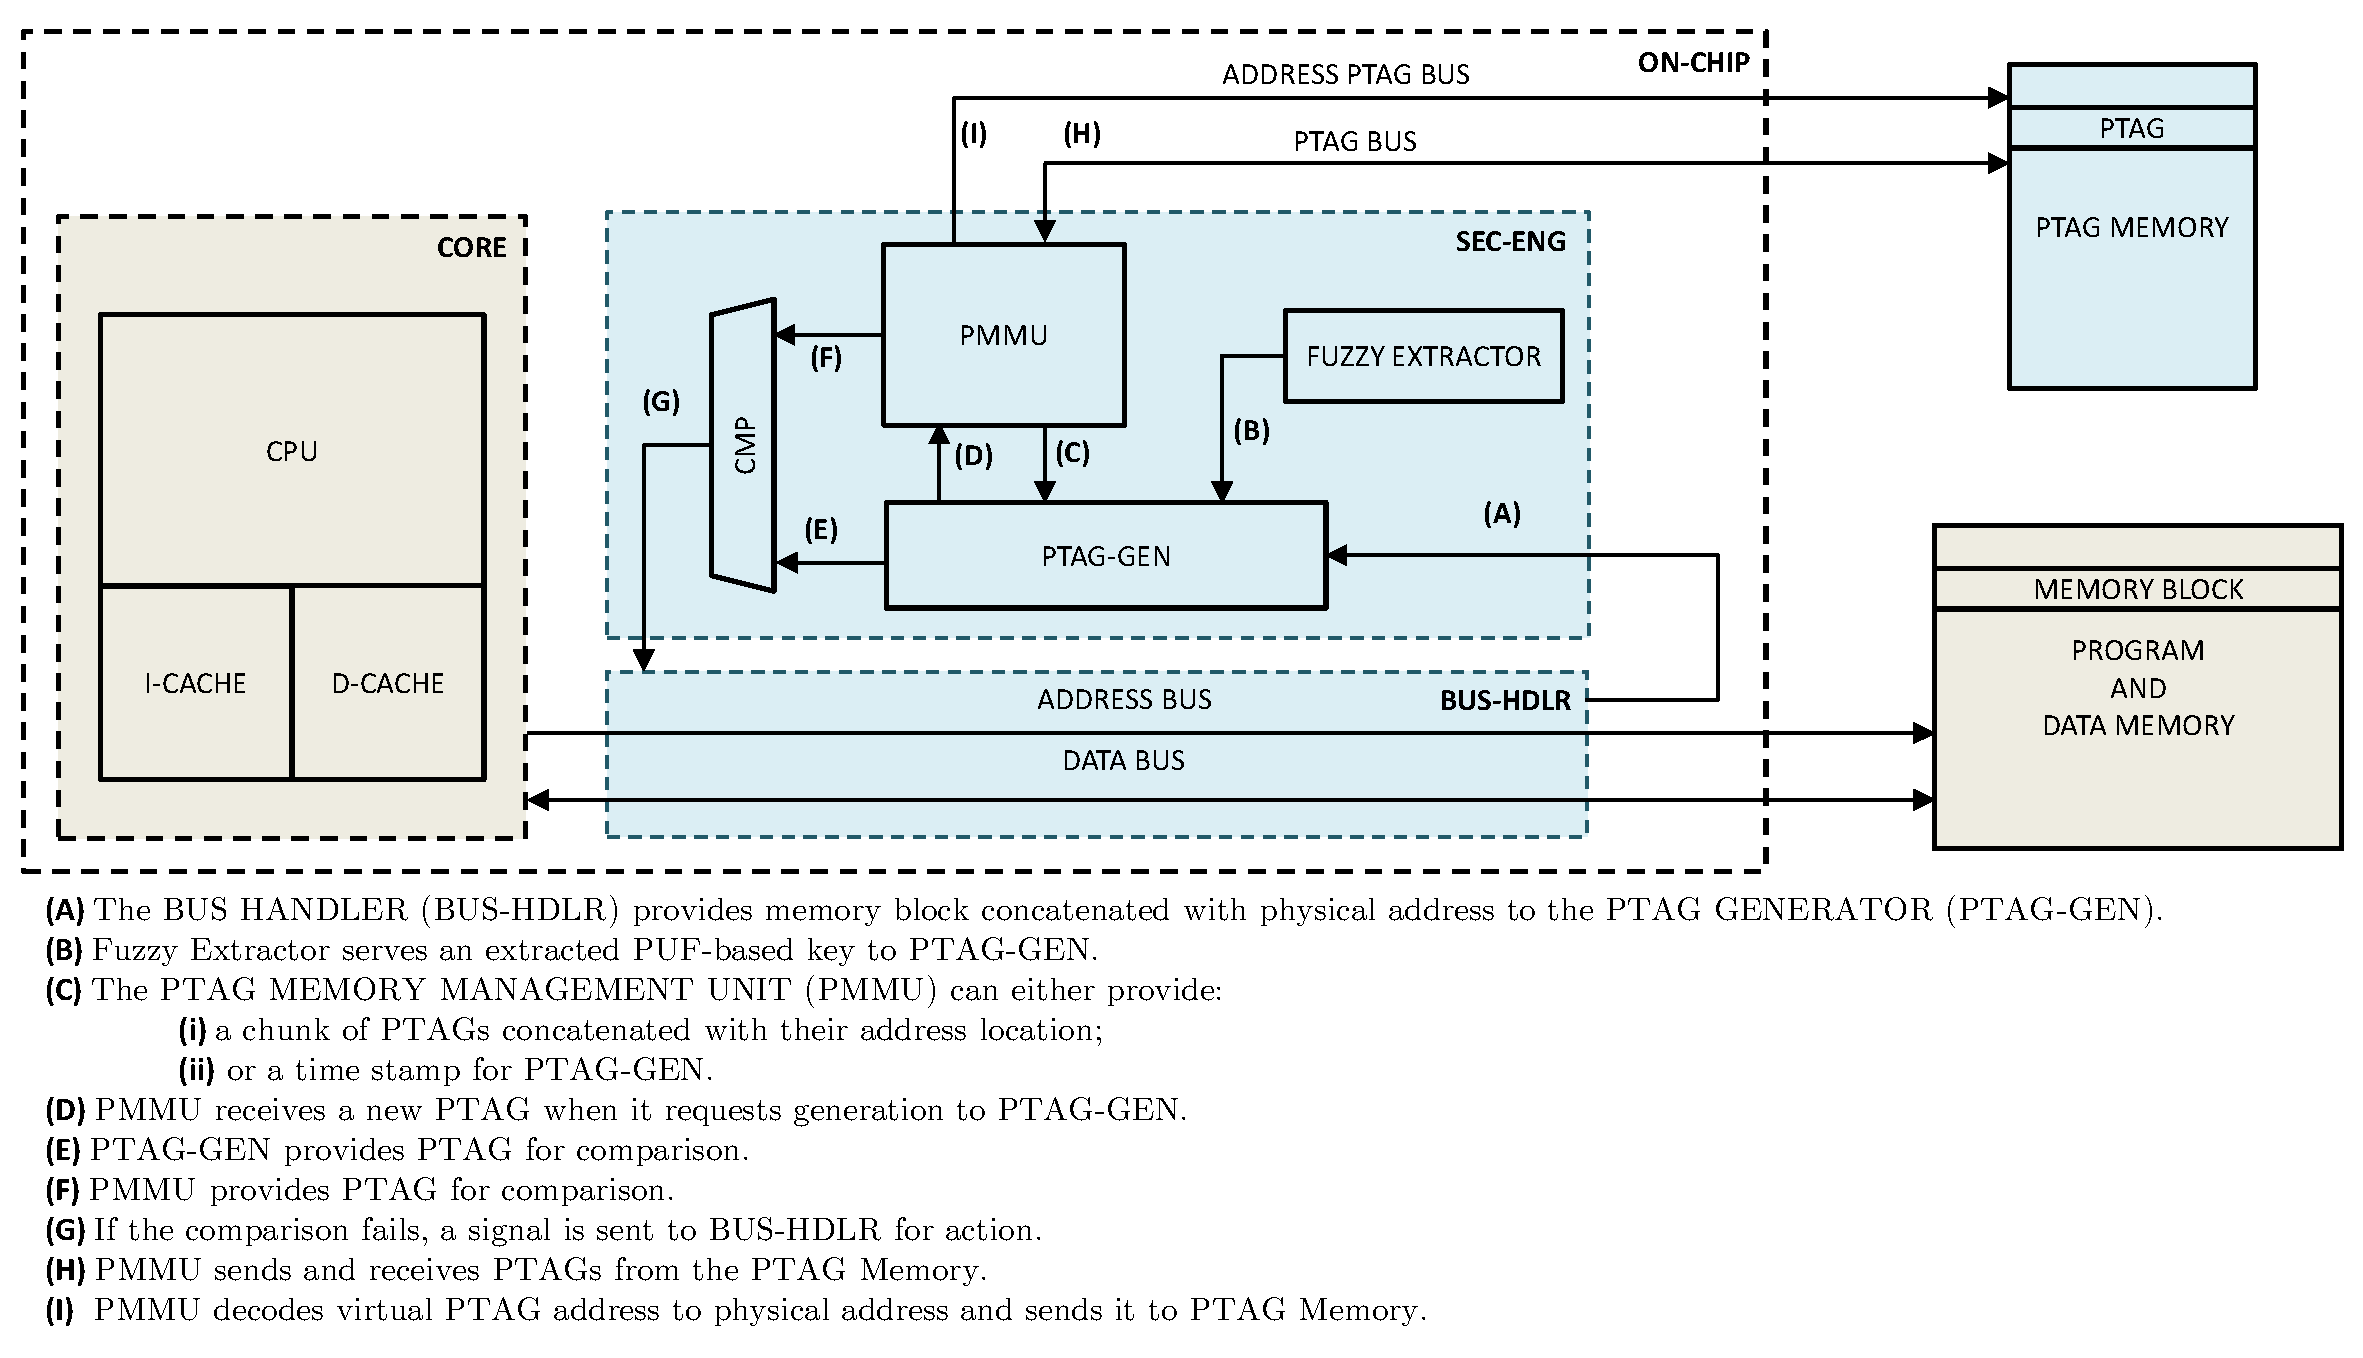
\includegraphics[scale=0.35]{cshia}
% %	\vspace*{-12pt} 
% 	\caption{A system overview of the \system~system.}
% %	\vspace*{-9pt} 
% 	\label{fig:system}
% \end{figure*}

  %\new{In comparison to traditional architectures, \system~includes two main modifications: The \textit{Secure Engine} (\tagsystem), which includes the \textit{PTAG Generator} (\ptaggen, Figure \ref{fig:ptaggen}); and the \textit{Security-Cache} (\seccache) that controls bus traffic between the processor and the \textit{Memory Controller} (\mctrl). Other two new architectural components are also required to complete the \system~design, the \textit{\ptag~Memory} and the \textit{PTAG Bus}. In a few words, when the processor requires\slash{}sends data\slash{}instructions to the \mctrl, the \seccache~sends the related cache line to the \tagsystem~for computing\slash{}validating its \ptag. Notice from Figure \ref{fig:system} that the \ptag~bus runs in parallel to the system buses, and thus no program can directly read the \ptag~Memory, since neither the processor nor the \mctrl~are aware about the \seccache.}


  % \subsection{\ptaggen~Operation}
  % \label{subsec:ptaggenOpr}

  % \new{The \tagsystem~controls the \ptaggen~based on the information delivered by the \seccache. This information is generated from bus transactions (Memory READ, Memory WRITE and I\slash{}O) between the processor and the memory controller, and which the \seccache~controls. Next, each \ptaggen~action is explained in regard to bus transactions.}
  
  %     \begin{figure*}[!ht]
	 %  \centering
	 %  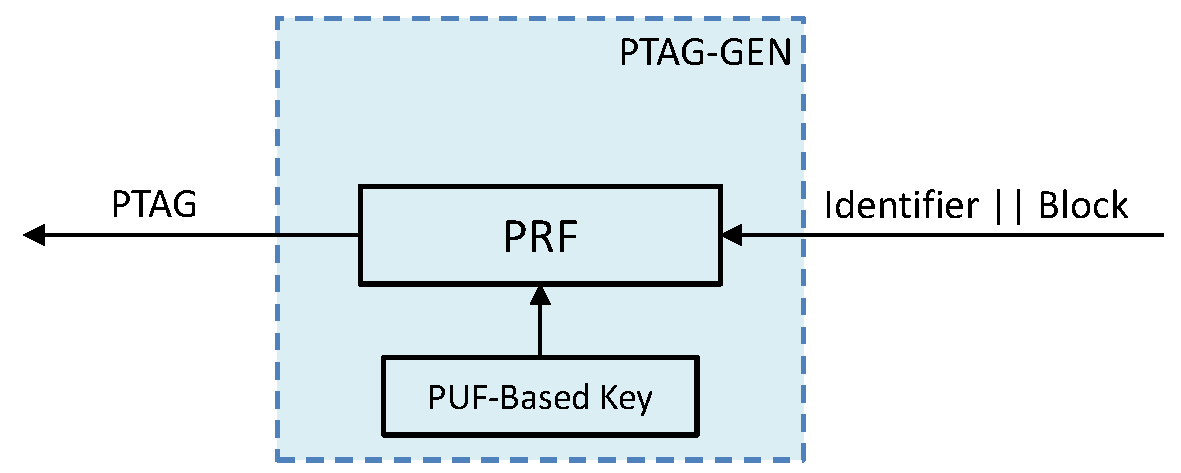
\includegraphics[scale=0.4]{ptaggen}
	 %  \caption{The \ptaggen~during \ptag~Generation (write) and \ptag~Verification (read) operations.}
  % %	\vspace*{-9pt} 
	 %  \label{fig:ptaggen}
  % \end{figure*}
  

	 %  \subsubsection{\ptag~Generation (memory write)}
	 %  \label{subsubsec:ptag-generation}
  % \new{During a write operation, the \seccache~passes data\slash{}instruction cache lines to the \tagsystem~and the \ptaggen~computes \ptags~and stores it into the \ptag~Memory. A \textit{Pseudorandom Function} (\prf) \cite{Goldreich2004} module is used to generate the \ptag~and takes as input the concatenation ($||$) of the cache line bits and the base address of the cache line provided by the core (see Figure \ref{fig:ptaggen}). In order to ensure uniqueness, the \prf~is configured using a \textit{unique-per-device key}. This key is produced by the intrinsic hardware features of a~\puf. Such authentication tag is specific to the core running that specific cache line, as ~\puf~outputs are dependent on the statistical variations of the manufacturing process, and are unique to each processor~\cite{Katzenbeisser2012}. Hence identical cache lines running on different processors will produce different \ptag~values for the same inputs. Notice that only code in the cache, for which integrity has been ensured, will be able to write to memory.}
  


	 %  \subsubsection{\ptag~Verification (memory read)}
	 %  \label{subsubsec:ptag-verification}
  % \new{During a read operation, the \seccache~passes data\slash{}instruction cache lines to the \tagsystem~and the \ptaggen~computes \ptags~for verification. As shown in Figure~\ref{fig:ptaggen}, during a read operation the cache line base address produced by the core is appended to the cache line contents read from memory and the result is fed to the \prf~module. The \ptag~produced this way is compared to the PTAG read from memory for equality. If the previously stored \ptag~and the recently computed value do not match, a \textit{Non-Maskable Interrupt} (NMI) is generated to the core (called \ptagnmi), as code\slash{}data integrity may have been violated. As shown in Figure \ref{fig:system}, in order to hide \puf~latency, the data\slash{}instruction is sent to the respective cache (I\$ or D\$) at the same time that \ptag-GEN computes the \ptag~for that cache line and compares it to its \ptag~previously stored into the \ptag~Memory.}

	 %  \subsubsection{Handling I\slash{}O}
	 %  \label{subsubsec:io}
  % In modern computer systems, I\slash{}O operations store data directly into specific memory regions through DMA mechanism. Thus, it is not possible to trust such memory regions and \system~does not ensure their integrity and authenticity. Software should first perform authentication of I\slash{}O data in a higher abstraction layer and then copy it to secure areas where the \system~can ensure integrity and authenticity.


\begin{figure*}[!ht]
	\centering
% 	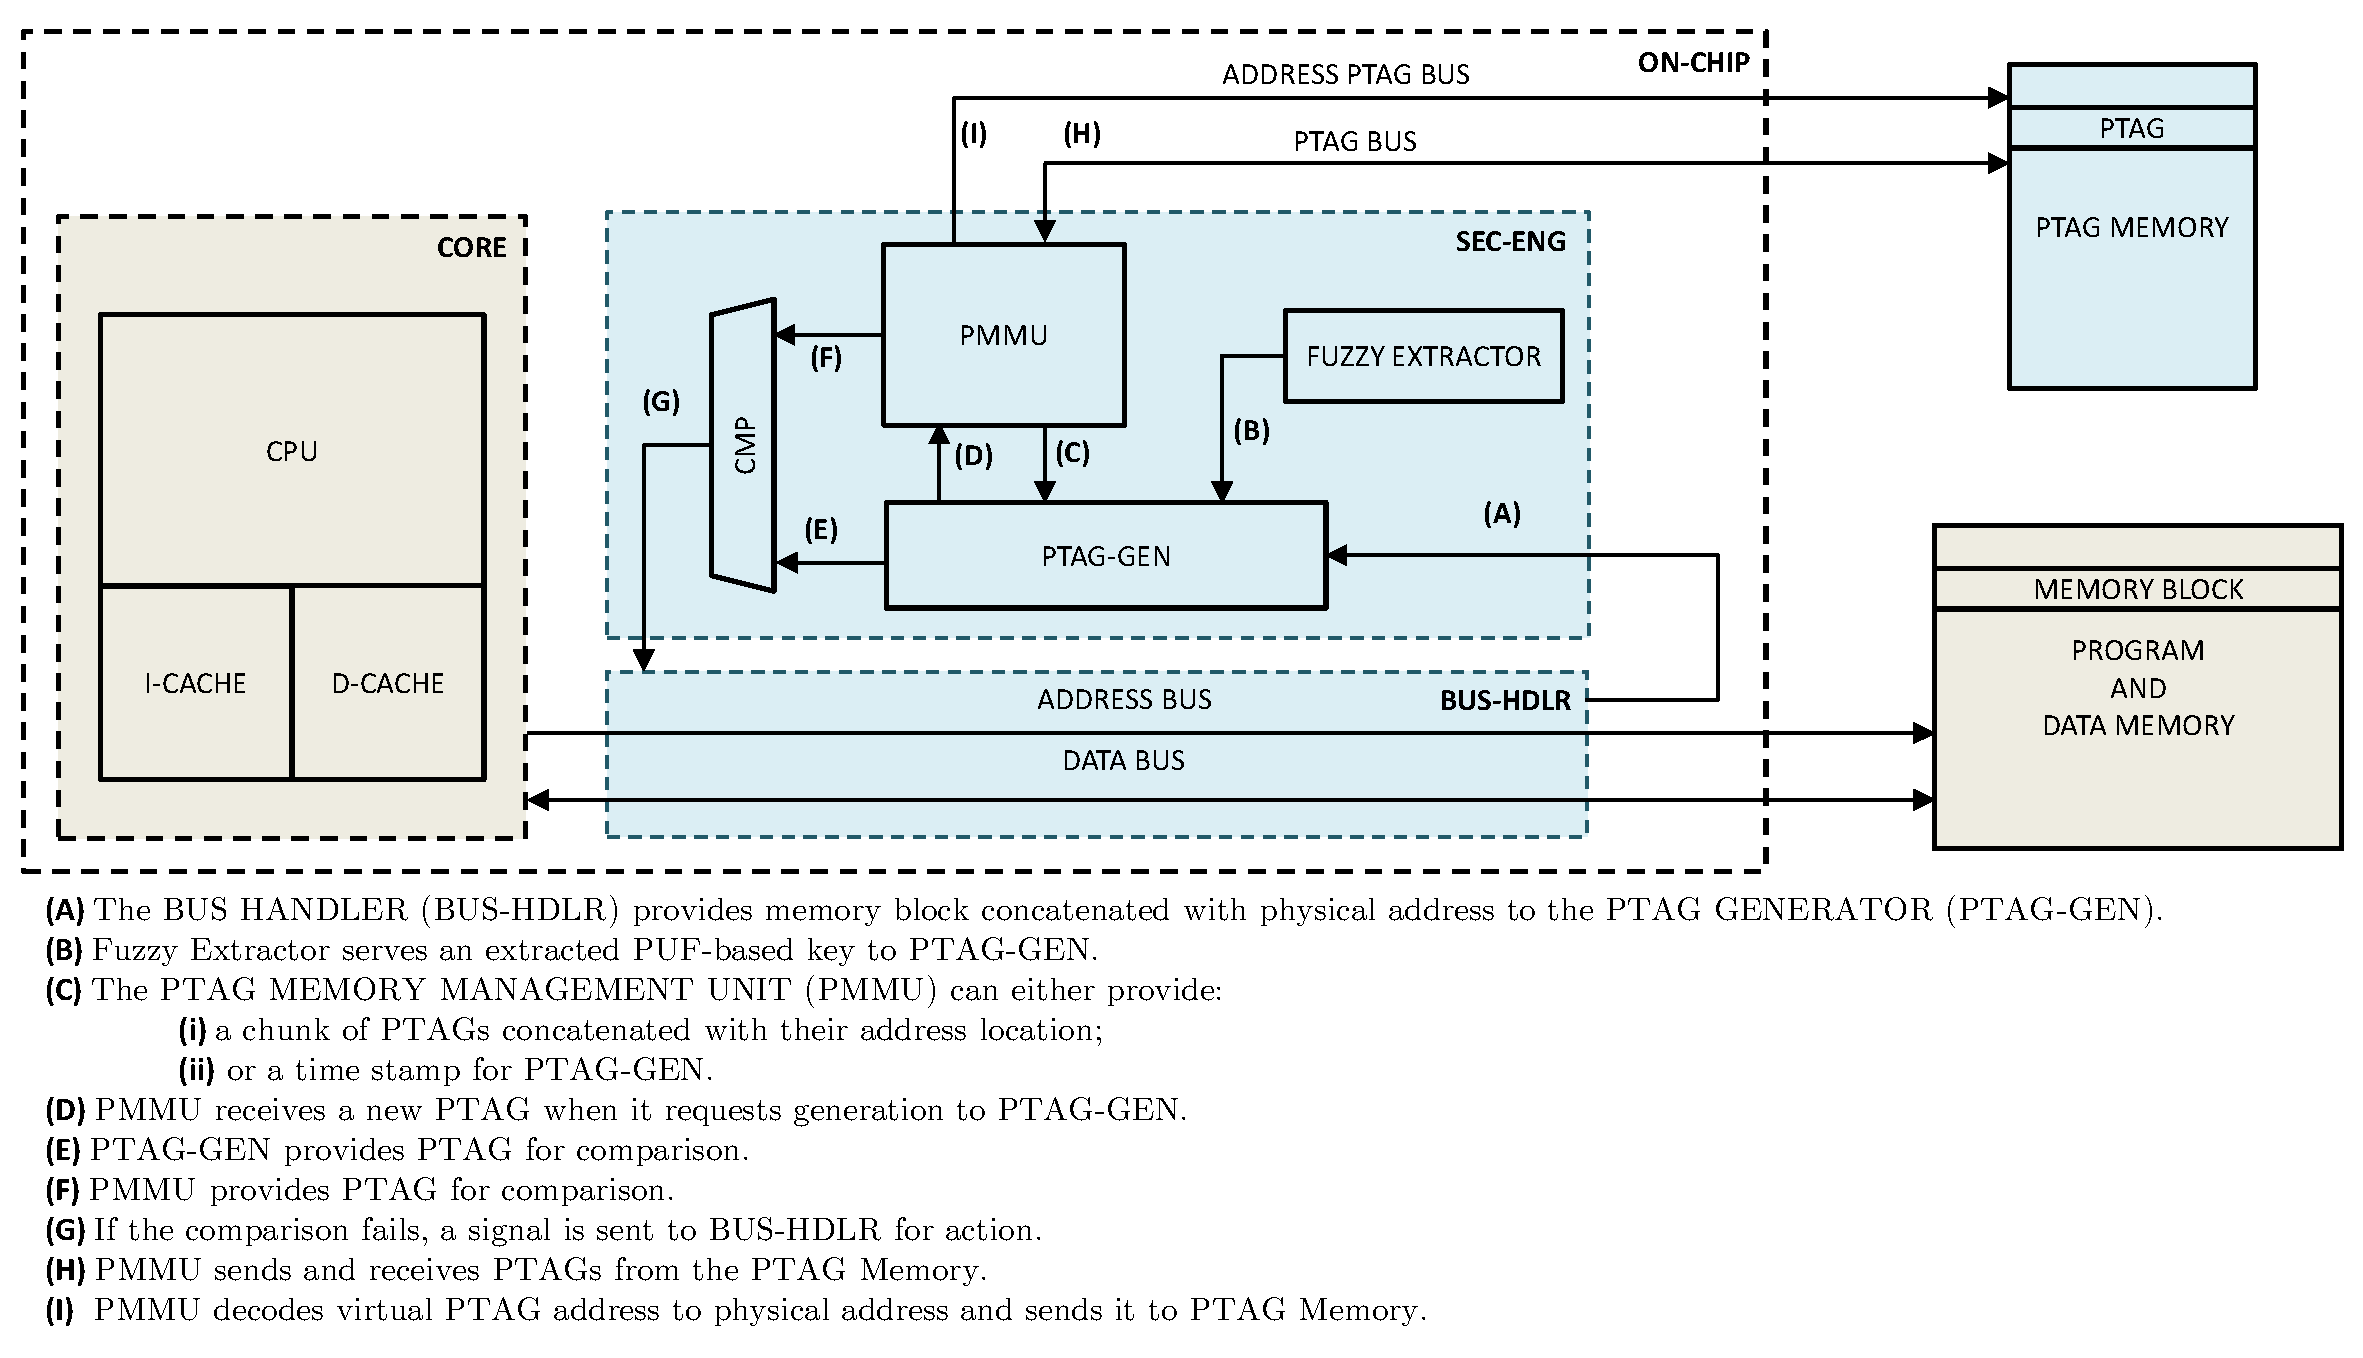
\includegraphics[scale=0.45]{cshia}
	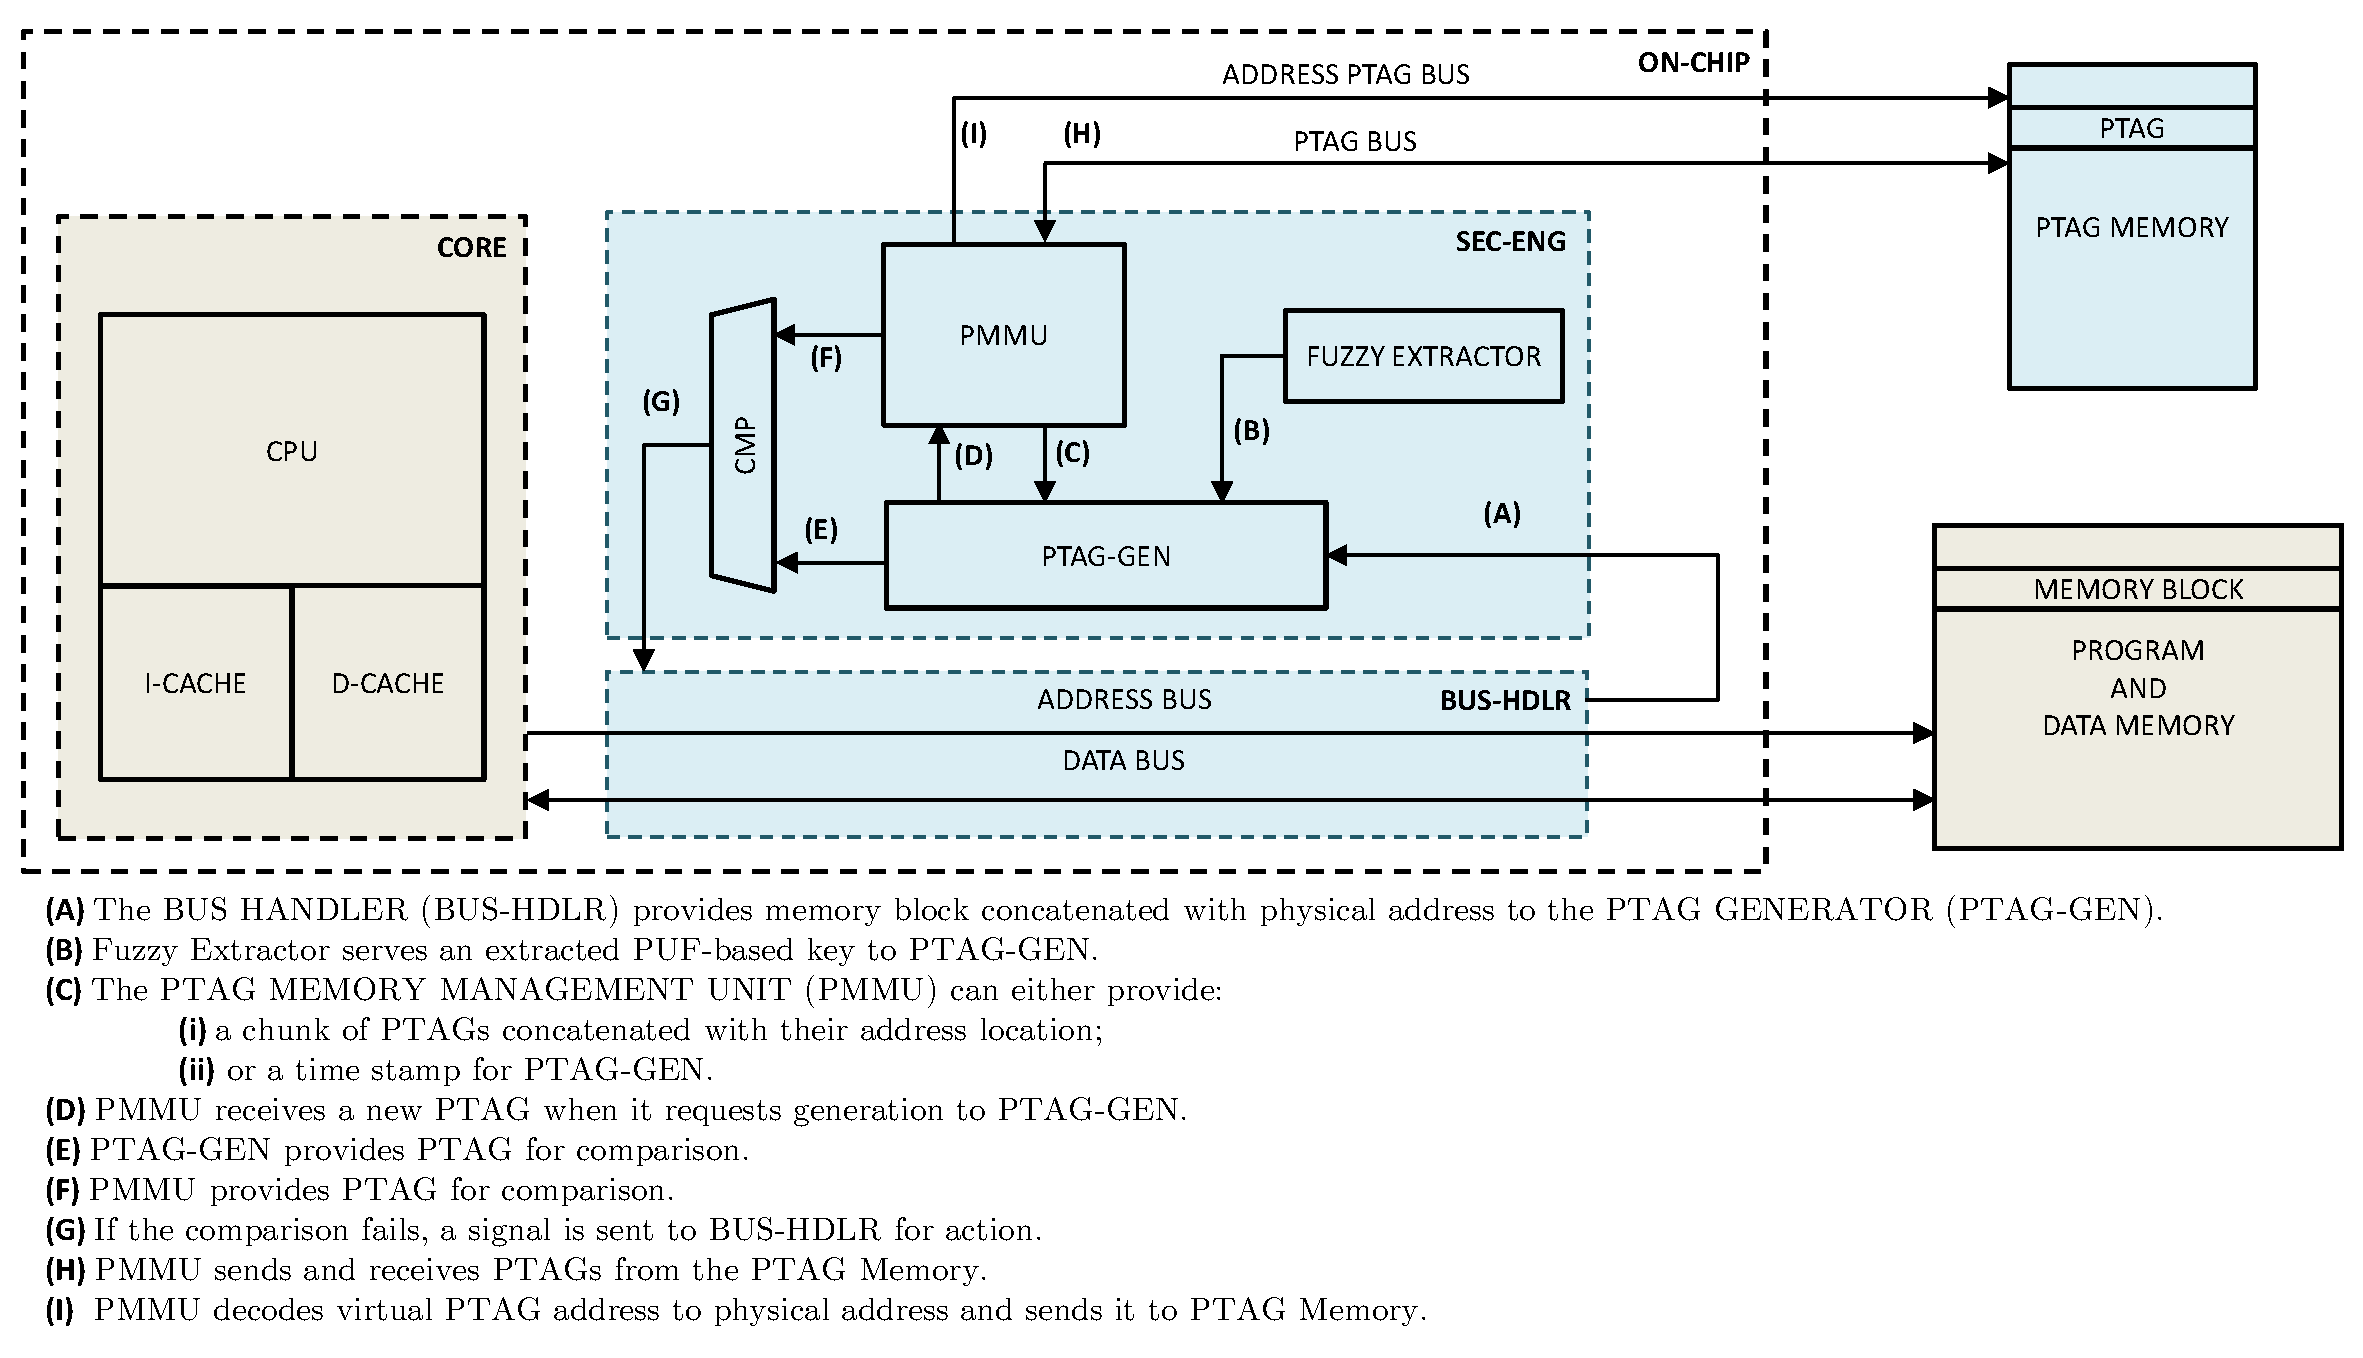
\includegraphics[width=\textwidth]{cshia}
	\caption{The \cshia~architecture.}
%	\vspace*{-9pt} 
	\label{fig:cshia}
\end{figure*}

\cshia~was originally proposed in \cite{Hoffman2015} as an architecture for \iot. However, we believe that \cshia~fits in a broader class of embedded system applications that can benefit from its nice security features. As we stated before, many embedded system applications do not need secrecy\slash{}confidentiality, but strongly require code and data authenticity and integrity. 
Using the original work with some architectural elements modified to provide stronger security features, the first LEON3 \fpga~ based implementation of \cshia was realized. This section focus on presenting our \cshia~implementation components and how they work to provide authenticity and integrity.

\section{Components of the Architecture}
\label{sec:Components-of-the-Architecture}
As Section \ref{subsec:integrity} discussed, the main resource to provide integrity are tags. Since \cshia~uses \puf-based keys to generate tags, we called them \puf-Tags, or \ptags~for short. \ptags~are the core of \cshia's design. They will be unique for each instance of \cshia~due to the unclonability property of \pufs. That ensures one-to-one relatioship between programs and instances, providing authenticity. To handle \ptags, three main components are added to a conventional embedded system architecture. They are: The \ptag~Memory; the Bus Handler (\handler); and the Security Engine (\seceng). Figure \ref{fig:cshia} shows this design and how components communicate between themselves. 

\ptag~Memory is an external memory and has its own buses. This architectural decision gives freedom to designers that can choose bus width, frequency, address space, etc. Because the processor is not aware of any additional component of \cshia, \handler~intercepts data transfers between processor and memory in order to provide them to \seceng~that generates tags. \handler~can also request data ( on behalf of the processor) to main memory so as  form complete memory blocks that are necessary to generate \ptags.

\seceng~has three major subcomponents. The main one is the \ptag~Generator (\ptaggen), which uses input data whose length is equal to a memory block concatenated with its address to generate \ptags. The \fuzzy~is only used when the system loses its secret key. For instance, after a power cycle. Thus, when the system is powered on, the \fuzzy~will extract the \puf-based key and provide it to \ptaggen. Finally, we have the \ptag~Memory Management Unit (\pmmu). The main functions of the \pmmu~are to store and request \ptags~from the \ptagmem~and also to decode internal addresses of \ptags~to physical addresses of \ptagmem. In addition to that, \pmmu~can have two distinct designs. If a designer chooses to use timestamps as solution for replay attacks, \pmmu~will have an internal memory to store and control timestamps of the memory blocks. However, if the solution for replay attacks is a \mt\cite{Elbaz2009}, \pmmu~will control verification and update of the tree, as well as it will have a cache memory, the \ptagcache, to speed up these tasks.


%\subsection{Bus Handler (\handler)}
%\label{subsec:handler}
%\lorenipsuns
%\subsection{Security Engine (\seceng)}
%\label{subsec:seceng}
%\lorenipsuns



%===========================================================================================================================================================

%======================================================
%Security Handler
%======================================================
\subsection{Bus Handler (\handler)}
This block has three main functions, monitoring the processor requests and respond then when necessary, 
assemble a line %explain better what line means
that can be multiple cache lines or any other combination necessary to be in the format
 of the security engine input  and prevent the processor the execute unsafe or unverified instructions
 as well as don't let  it  write in the bus any unsafe operation.
%======================================================
%Block Diagram
%======================================================
\subsubsection{Block Diagram}

\begin{figure*}[!ht]
	\centering
	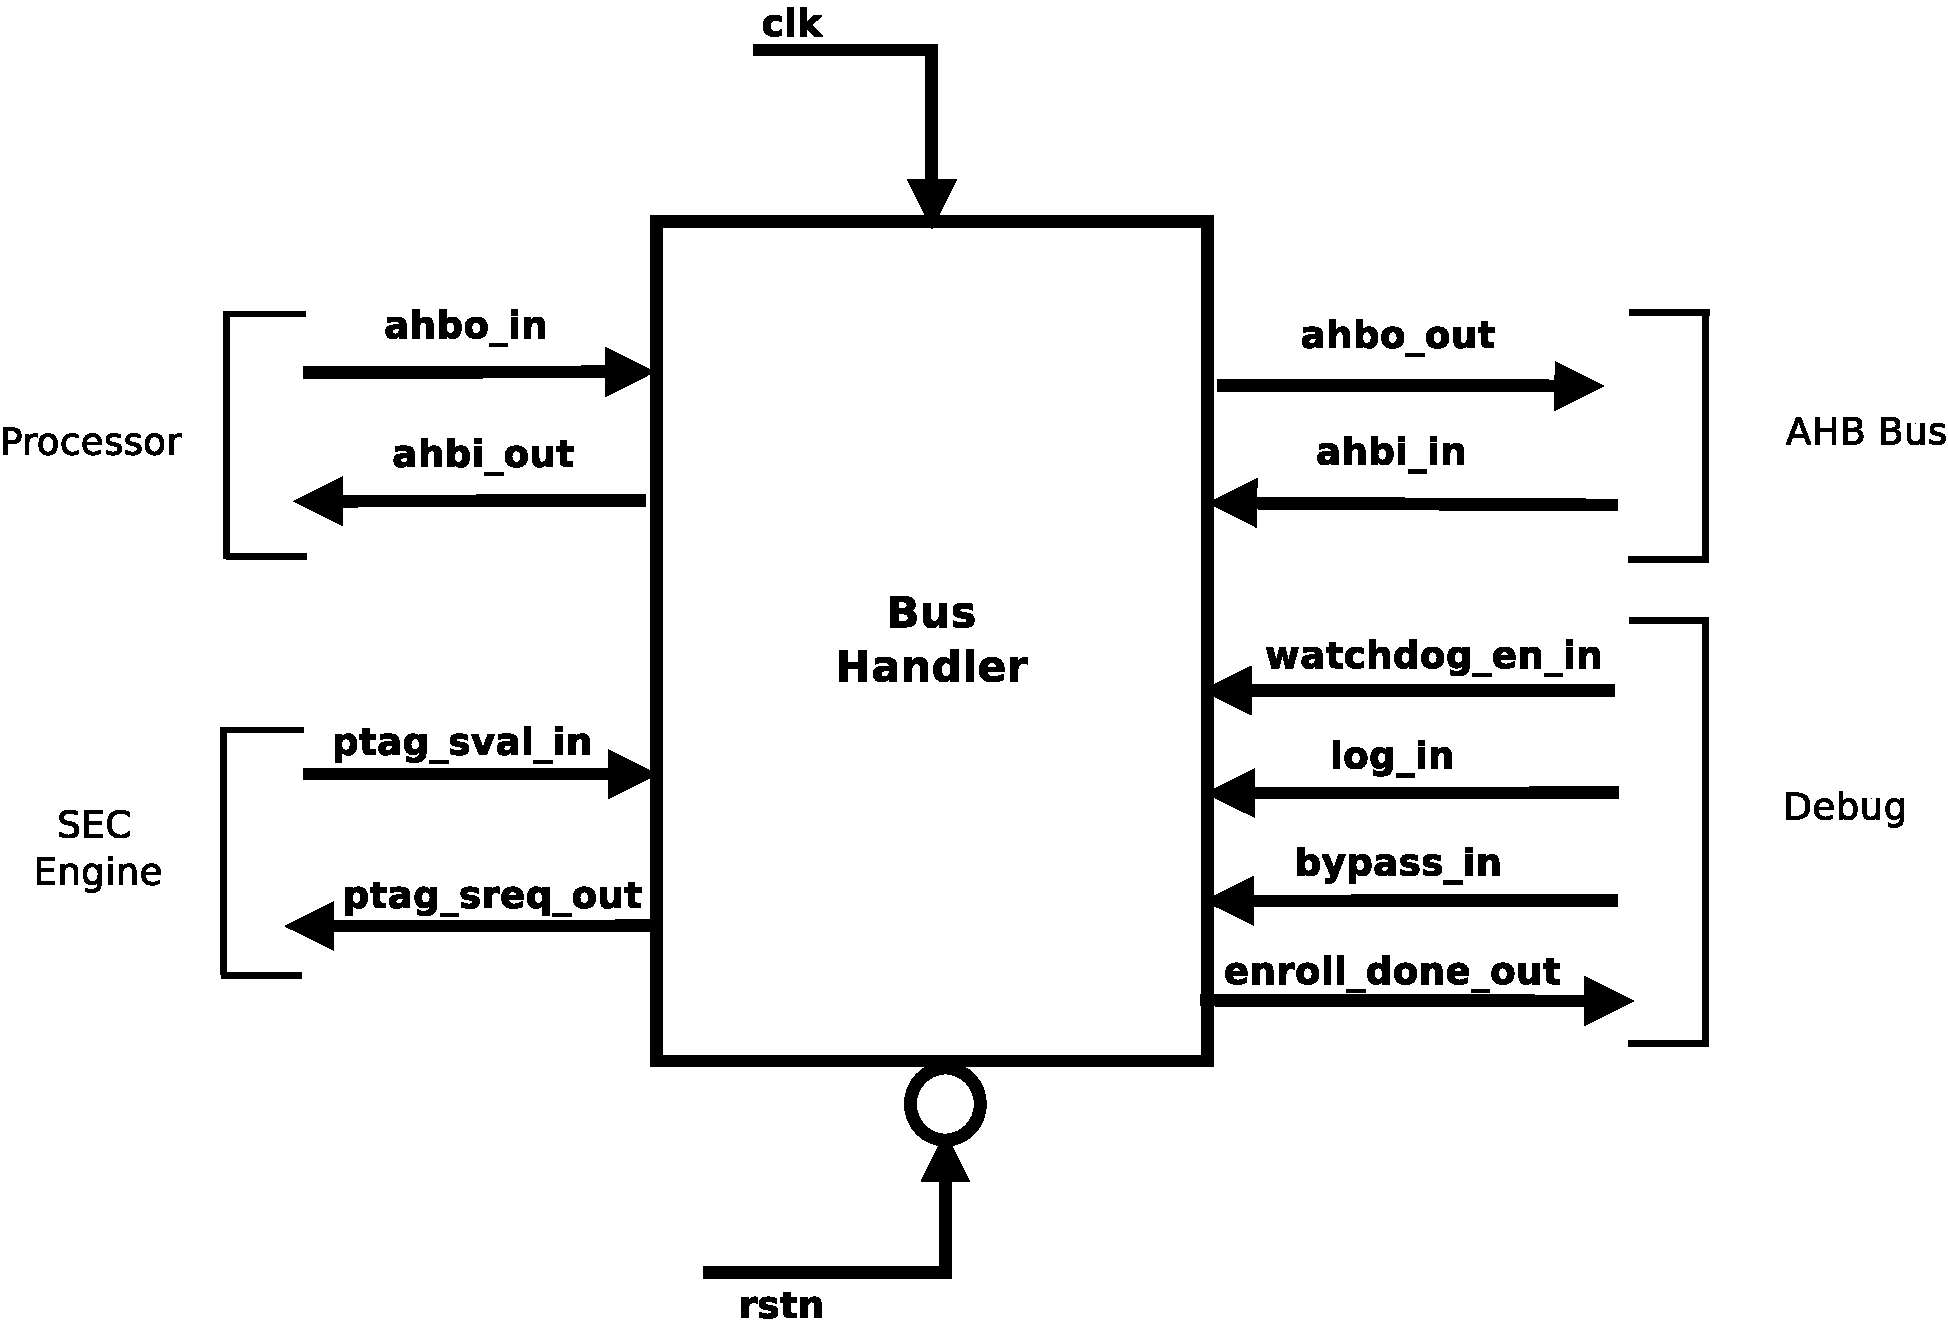
\includegraphics[scale=0.45]{bus_handler}
    \caption{Bus Handler  black box  }
%	\vspace*{-9pt} 
	\label{fig:bhbb}
\end{figure*}


%======================================================
%Signal Description
%======================================================
\subsubsection{Signal Description}

The inputs and outputs of this block can be split in three interfaces and control being
the signals  ahbo\_in and ahbi\_out the interface with the LEON3 processor,  ahbo\_out  and ahbi\_in
the interface with the bus , ptag\_sval\_in and ptag\_sreq\_out with the security engine  and control
 the signals clk ,reset\_n and bypass\_in.
 The description of each type can be found in the Appendix \ref{ap:signals}.
\begin{table}[H]
\centering
\label{table:shports}
\begin{tabular}{l l l l}
\textbf{Port}   & \textbf{in/out} & \textbf{Type}        & \textbf{Description} 	\\ \hline \hline
clk             & in              & std\_ulogic          & system clock         	\\ \hline
rstn            & in              & std\_logic           & negated rset         	\\ \hline
bypass\_in      & out             & std\_logic           & bypass input         	\\ \hline
ptag\_sreq\_out & out             & ptag\_sec\_req\_type & security check request    	\\ \hline
ptag\_sval\_in  & in              & ptag\_sec\_val\_type & security check response  	\\ \hline
ahbi\_in        & in              & ahb\_mst\_in\_type   & AHB input from bus      	\\ \hline
ahbi\_out       & out             & ahb\_mst\_in\_type   & AHB output to processor      \\ \hline
ahbo\_in        & in              & ahb\_mst\_out\_type  & AHB input from processor    \\ \hline
ahbo\_out       & out             & ahb\_mst\_out\_type  & AHB output to BUS            \\ \hline
\end{tabular}
 \caption{Ports of the security handler}
\end{table}





\subsubsection{Functional Description}

%   \begin{figure}[H]
%     \centering
%     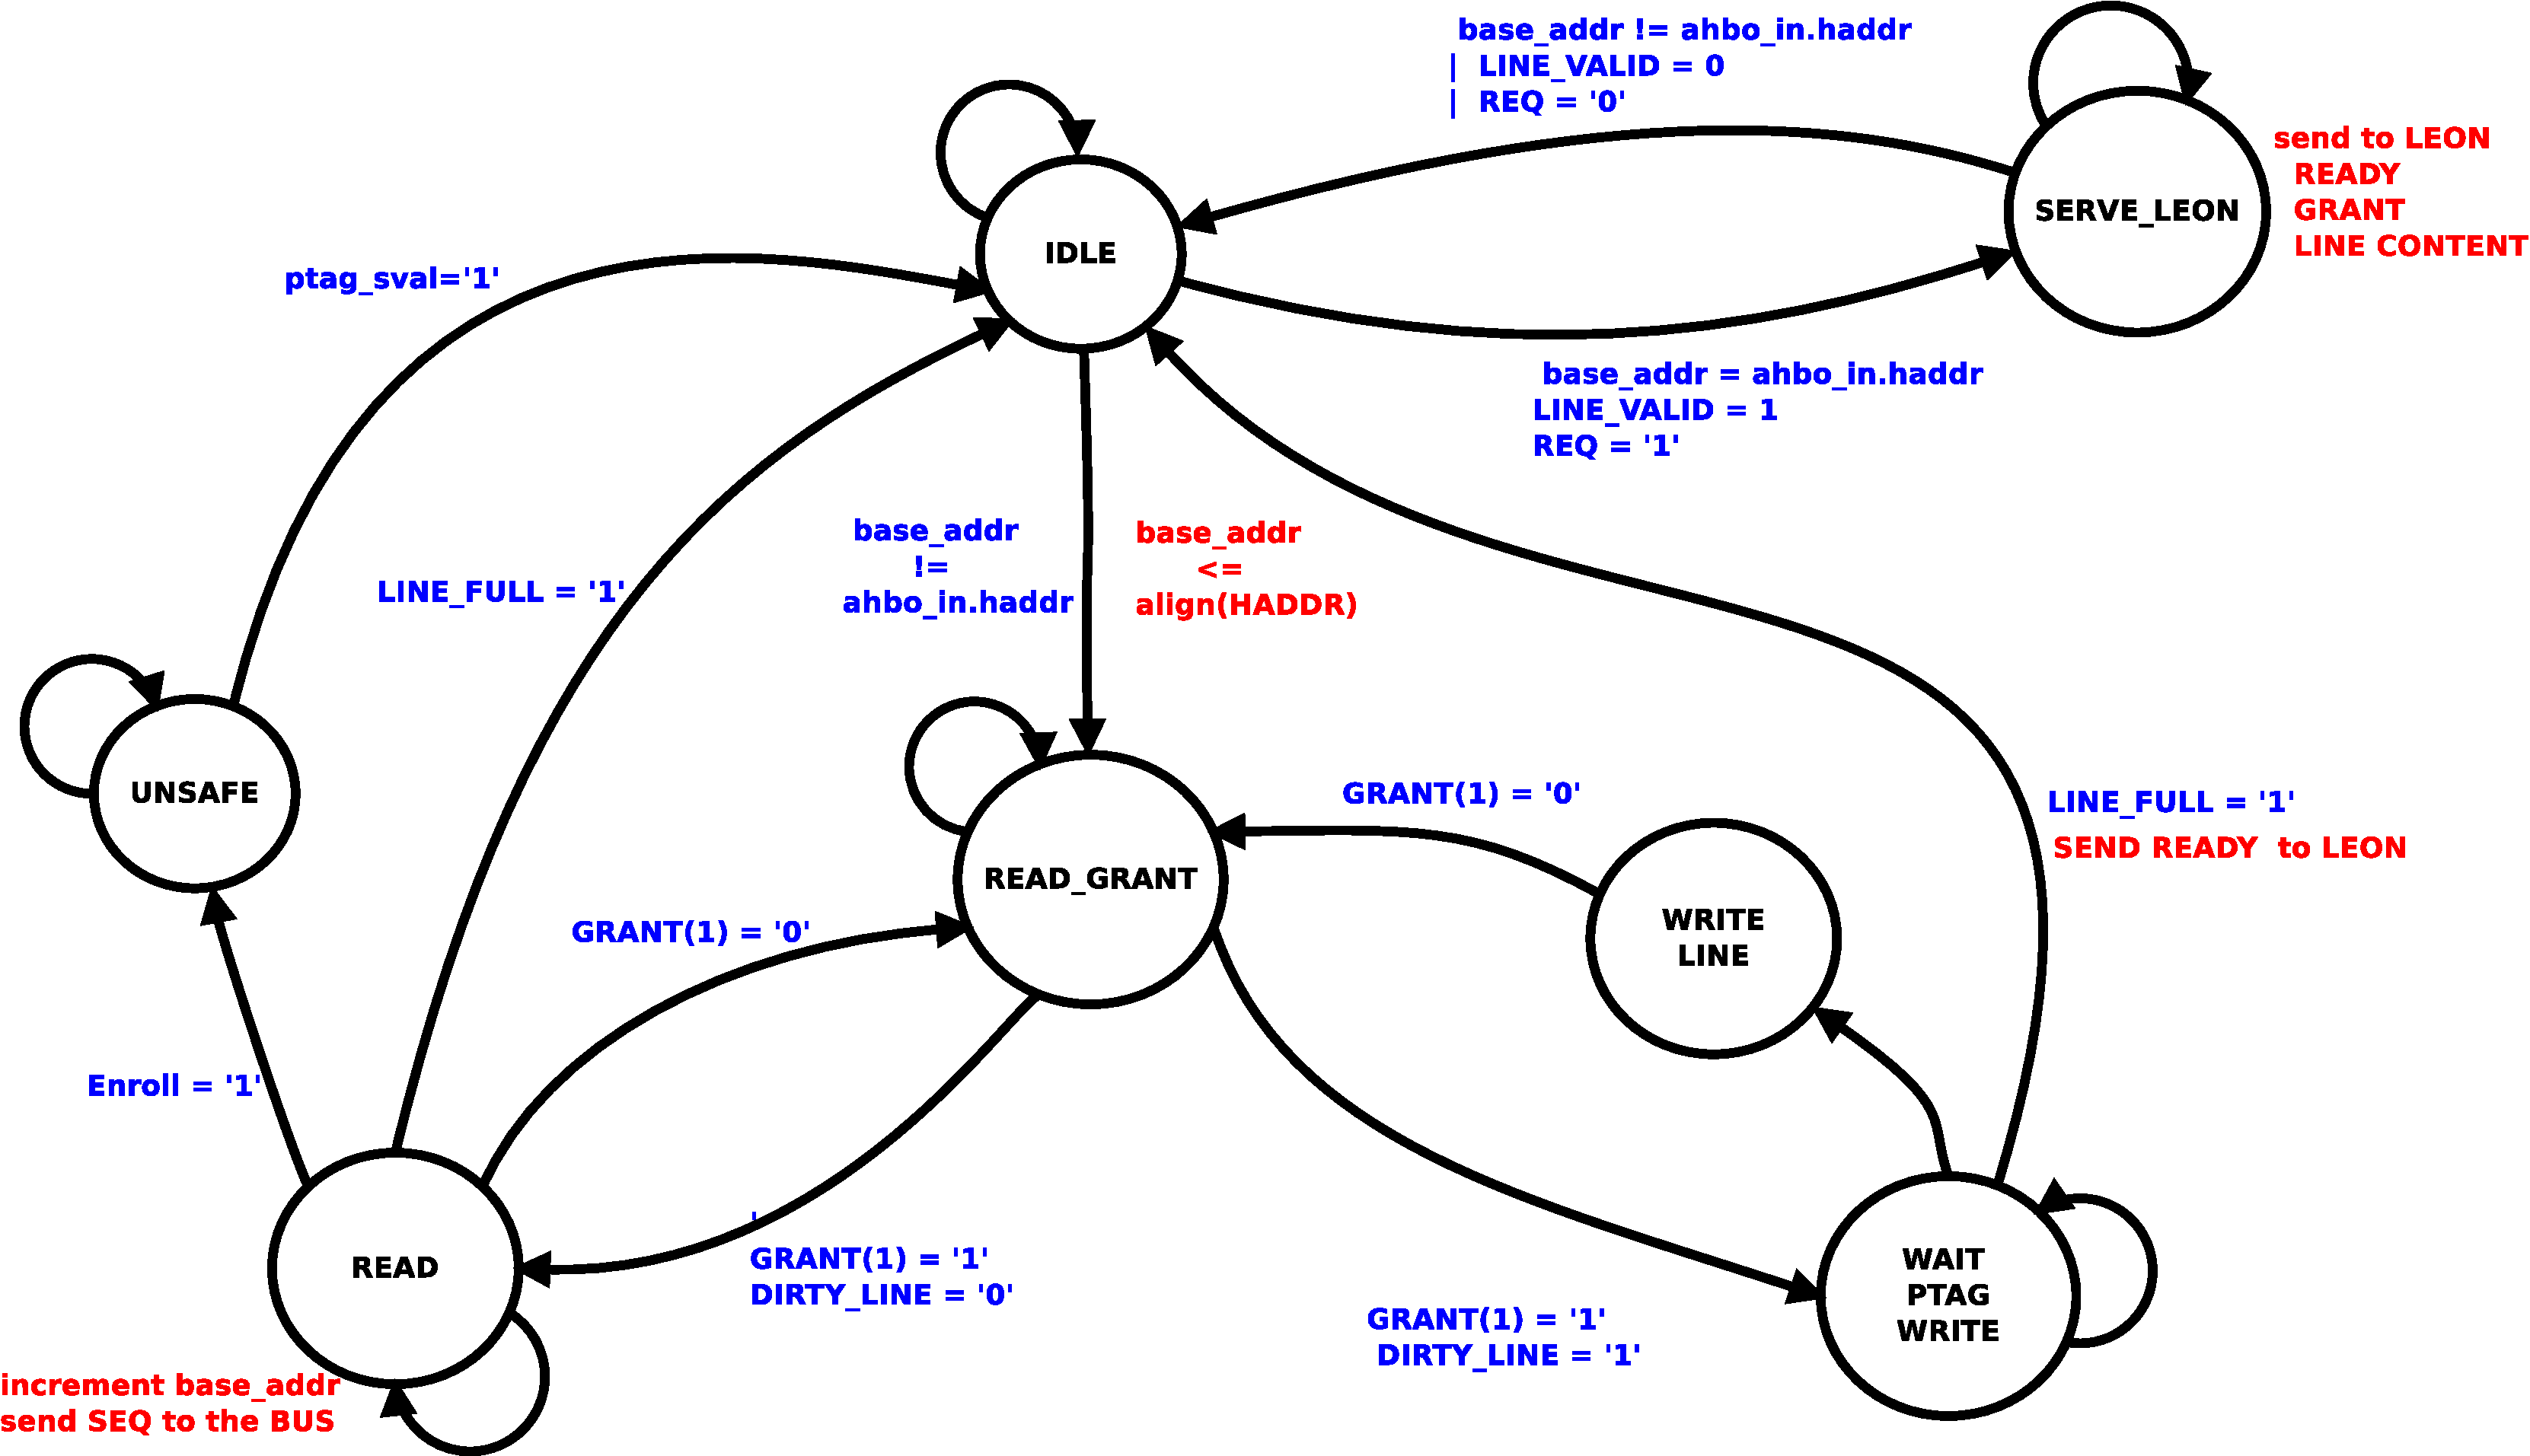
\includegraphics[width=0.85\textwidth]{Figures/pdf/sec_hand_state_machine.pdf}
%     \caption{Top of the system  }
%     \label{fig:phsm}
% \end{figure}
\begin{figure*}[!ht]
	\centering
	\includegraphics[scale=0.45]{sec_engine_sm}
    \caption{Bus Handler state machine  }
%	\vspace*{-9pt} 
	\label{fig:phsm}
\end{figure*}
Since this  state machine controls all the operations of the security handler the functional 
description of this block can be explained using the state transactions of Figure \ref{fig:phsm} and the 
following state description:

\begin{itemize}
 \item{\textbf{IDLE}}
 
 The system stay in this state  until the processor signalizes a request, given the request 
 there are three options, the line contains the content requested by the processor, in this case
 the request can be responded in the SERVE LEON state, the line does not contain the content required
 so a new line must be loaded in the READ GRANT state or the current line is not safe and the system will halt
 going to UNSAFE state.
 
  \item{\textbf{READ GRANT}}
  
  This state is required for any transaction in the bus, it requests the bus grant for the arbiter prior to 
  begin the request, once the arbiter gives the grant the line status is checked and if the line is dirty( the processor
  update any value in the line) then it needs to be written in the memory before loading a new line, if this is the case
   then the system goes to WRITE LINE state, if no changes were made in the line then a new line is loaded in the READ LINE 
   state. The steps needed to acquire the bus grant are shown in section \ref{op:grant}.
  
  \item{\textbf{READ LINE}}
  
  
  A new line will be loaded from the main memory to the local buffer,the  steps needed to execute
   a read or write operation is shown  in \ref{op:rw}, so a counter is started and counts the 
  number of words the bus provided, so when the line is loaded the line status is changed to valid and
  the system goes back to IDLE state. When  the line is ready  then a request is sent to the security engine 
  to check if the line is safe and the system will freeze until the integrity of the line is confirmed.

 \item{\textbf{WRITE LINE}}
 
 Once the line is dirty and need to be written in the main memory, a counter is  starded, similar to the read process 
 but it now counts each time the write request is confirmed by the bus, when all words were written  the line sirty status 
 is now changed to not dirty and the system goes to IDLE. In the process of writing the line to memory, in parallel a request is made 
 to the security engine to calculated the new PTAG related tohis line and store it in the PTAG memory.

 \item{\textbf{SERVE LEON}}

 On this state  all LEON requests  read or write are executed, if the content needed is  in the line. 
 when any operetaion requires a word  that is not in the local line buffer then the system  goes back to IDLE state.
 
 
 \item{\textbf{UNSAFE}}
 
 
When a security check fails  on the IDLE state the system uses this as a trap state to halt.

\end{itemize}




\subsubsection{subsection}{Operation}

% \begin{subsubsection}{Requesting Grant}
% \label{op:grant}


%   \begin{figure}[H]
%     \centering
%     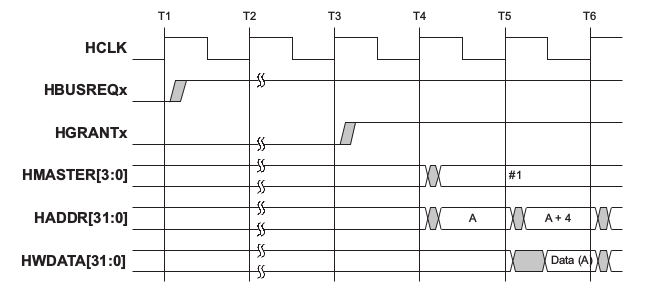
\includegraphics[width=0.95\textwidth]{Figures/others/grant_nowait.png}
%     \caption{Requesting grant with no wait states  }
%     \label{fig:gnwsm}
% \end{figure}


%   \begin{figure}[H]
%     \centering
%     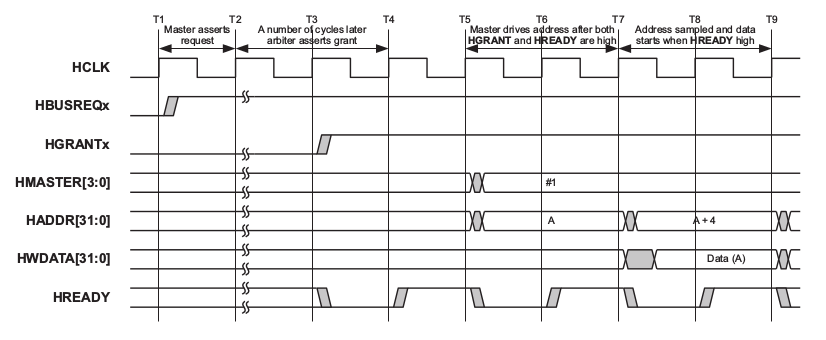
\includegraphics[width=0.95\textwidth]{Figures/others/grant_wait.png}
%     \caption{Requesting grant with wait states  }
%     \label{fig:gwsm}
% \end{figure}
% \end{subsubsection}

% \begin{subsubsection}{Read and Write BUS Operations}
% \label{op:rw}


%   \begin{figure}[H]
%     \centering
%     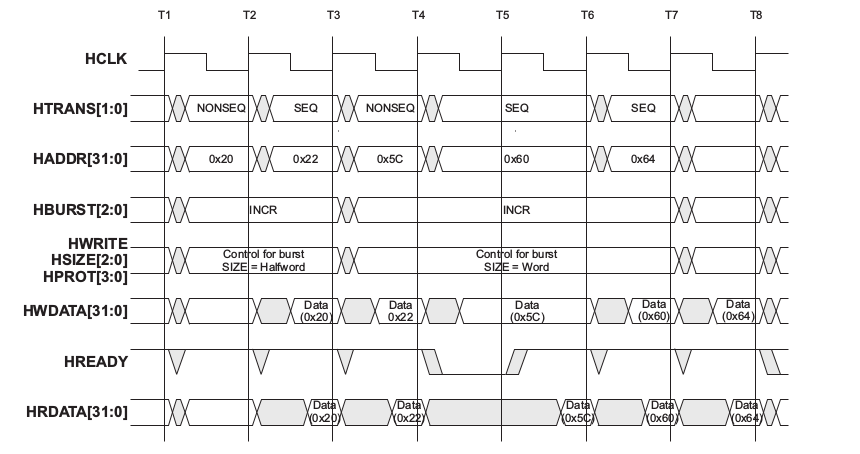
\includegraphics[width=0.95\textwidth]{Figures/others/undef_burst_length.png}
%     \caption{burst transfer with undefigned lengths read and write }
%     \label{fig:ublsm}
% \end{figure}

% \end{subsubsection}

% \end{subsection}
% \end{section}




%======================================================
%Security Engine
%======================================================
\subsection{Security Engine}

This block is responsable for the interface with the external memory wich stores the physical tags values
for each sets of challenges, and for calculatng this values using one or more PUFs, the PUF description is in section XX.


\begin{figure*}[!ht]
	\centering
	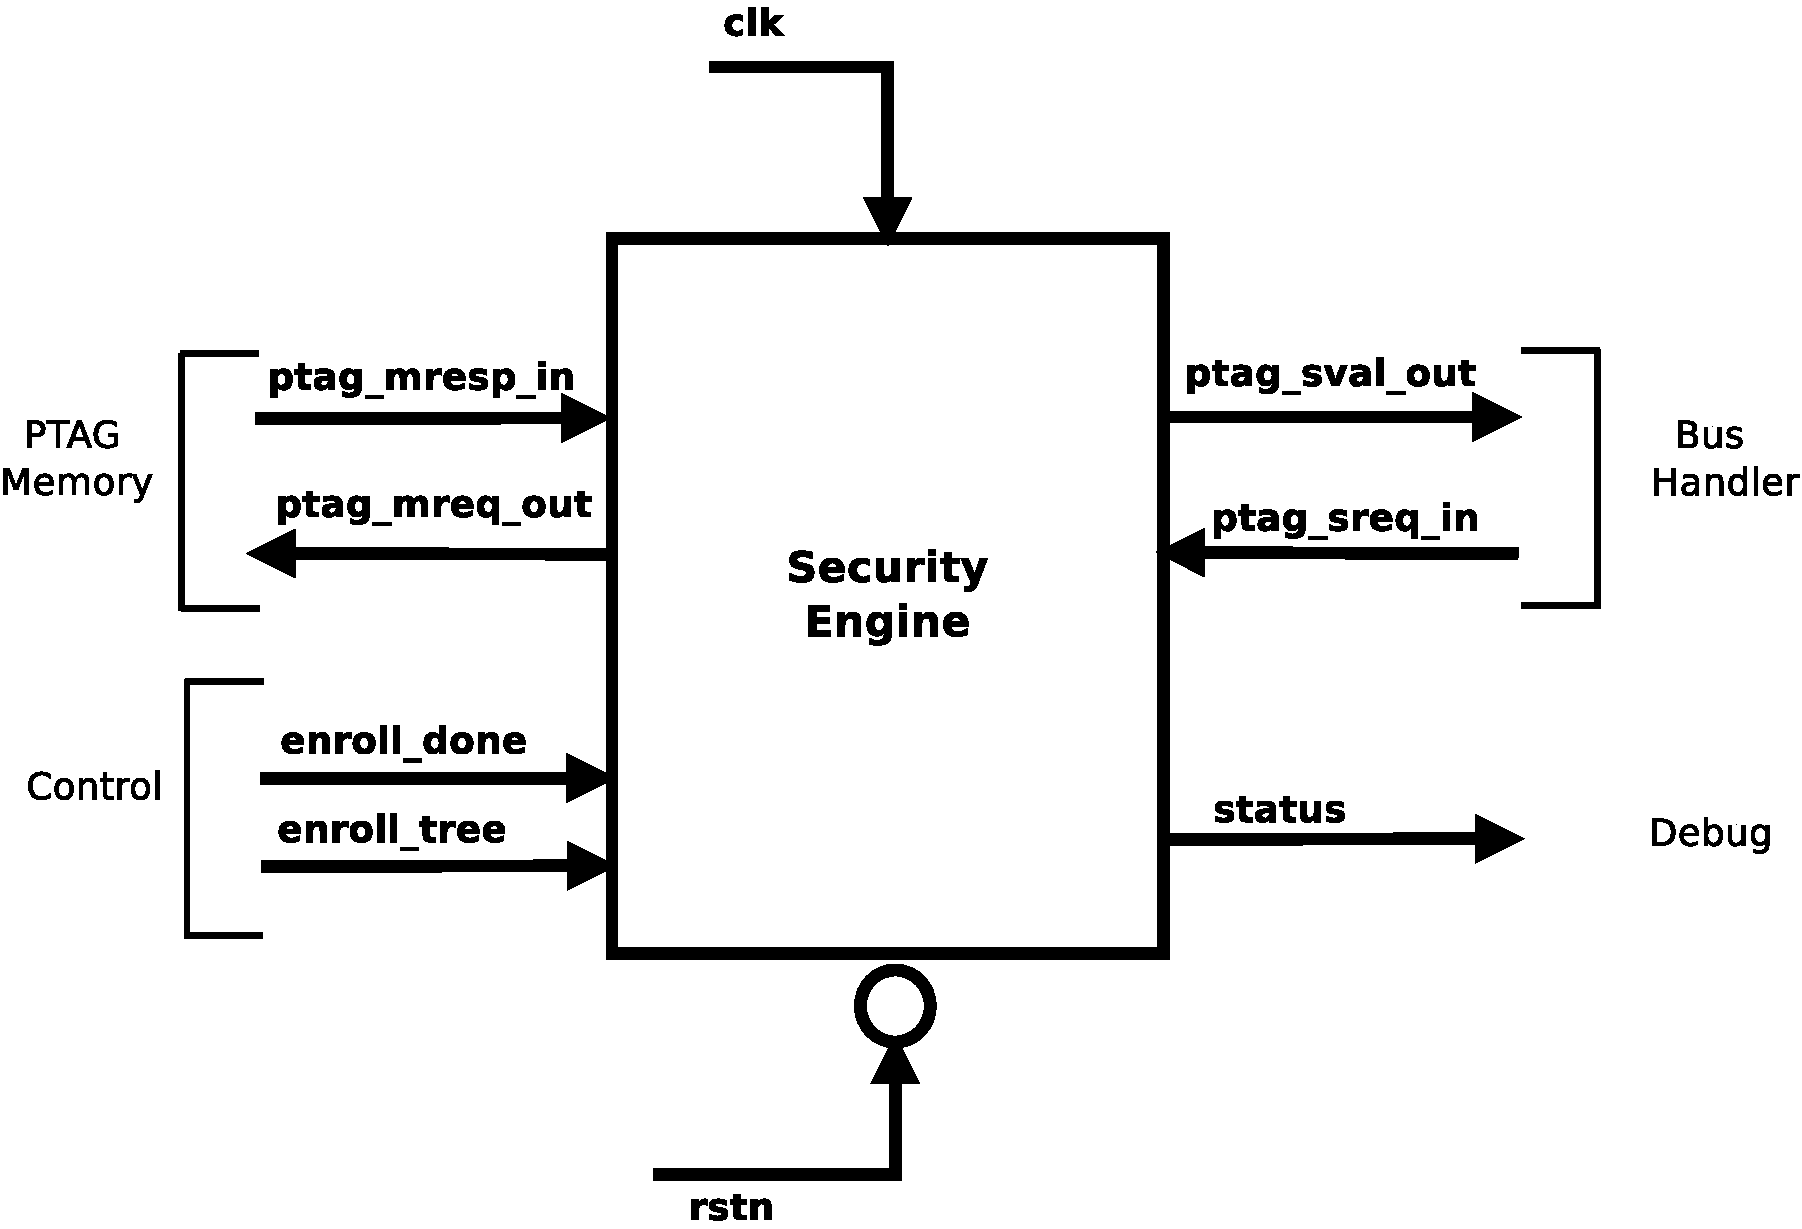
\includegraphics[scale=0.45]{security_engine_bb}
    \caption{Security engine  black box  }
%	\vspace*{-9pt} 
	\label{fig:sebb}
\end{figure*}




\subsubsection{Signal Description}

\begin{table}[H]
\centering
\label{table:seports}
\begin{tabular}{l l l l}

\textbf{Port}   & \textbf{in/out} & \textbf{Type}        & \textbf{Description} 	\\ \hline \hline
clk             & in              & std\_ulogic          & system clock         	\\ \hline
rstn            & in              & std\_logic           & negated reset         	\\ \hline
ptag\_sreq\_in  & in              & ptag\_sec\_req\_type & security check request    	\\ \hline
ptag\_sval\_out & out             & ptag\_sec\_val\_type & security check response  	\\ \hline
ptag\_mreq\_out & out             & ptag\_mreq\_type 	 & ptag memory  request    	\\ \hline
ptag\_mresp\_in & in              & ptag\_mresp\_type 	 & ptag memory  response  	\\ \hline
\end{tabular}
 \caption{Ports of the security engine}
\end{table}




\subsubsection{Functional Descricption}
  \begin{figure}[H]
    \centering
    \includegraphics[width=0.90\textwidth]{figures/pdf/sec_engine_sm.pdf}
    \caption{Top of the system  }
    \label{fig:sesm}
\end{figure}


The functional operation of this block consists in two basic actions, given a challenge
calulate the PTAG  using the internal PUF  and if this is a check operation the compare
 the calculated value with the equivalent from the PTAG memory, if its a write operations
 than just store the calculated value in the PTAG memory.the state machine needed to complete
 this task is described bellow.

\begin{itemize}
  \item{\textbf{IDLE}}
 
The security engine stays in  IDLe  until a valid challenge is siganlized, then the input is 
registered and a request for the PUF is sent to calculate tha PTAG , as well as read operation 
 to the PTAG memory  in case of a check operation.
 
  \item{\textbf{CALC PTAG}}
  When  a new challenge comes to be checked or written, a new ptag is calculated using the internal PUF, 
  after the calculation is ready the controller goes either to VALIDATE state if this is a check operation
  or to WRITE PTAg state if this is a write operation.
  

  \item{\textbf{VALIDATE}}
  Since in this state the PTAG from the PTAG memory and the calculated from the PUF are ready this state compares
  the values and send the result as a security response to the security handler. Then  the system goes back to IDLE.
  

 \item{\textbf{WRITE PTAG}}
 This state  uses the memory interface to  write the calculated PTAG in the PTAG memory and send a confirmation
 through the security response to the security handler.



\end{itemize}


%===========================================================================================================================================================




\subsection{Memory Management Unit (\pmmu)}
\label{subsec:pmmu}
\lorenipsuns

\subsection{\ptagmem}
\label{subsec:ptagmem}
\lorenipsuns



\section{Operation Modes}
\label{sec:opmodes}

%describe all


\subsection{Runtime Phase}
\label{subsec:runtimephase}
\def\fenroll{Figure \ref{fig:fuzzy-extractor} \subref{fig:fuzzy-enroll}}
\def\fregen{Figure \ref{fig:fuzzy-extractor} \subref{fig:fuzzy-regen}}
After the enrollment phase, \cshia~instances are ready for distribution.Here is how \cshia's components work together. \handler~checks for memory read-write operations of the processor. When it perceives a memory read it will capture memory words \andor~request memory words to compose a memory block. Then it sends this memory block and its address to \seceng. On its turn, \seceng~uses \pmmu~to bring the corresponding \ptag~of that memory block from \ptagmem, while \ptaggen~computes a \ptag~using the content served by \handler. After that, the \ptag~brought from \ptagmem~and the one computed are compared. If they match, \seceng~knows that neither the \ptag~nor the memory block were tampered with. Otherwise, \seceng~alerts the handler that can isolate the processor or sends a non-maskable interrupt to the processor.


For write operations, the process is simpler. Once any memory block that reached the processor was verified for integrity and authenticity, \handler~can serve the cache line to \seceng~that uses \ptaggen~to compute a new \ptag~and \pmmu~sends that \ptag~to \ptagmem.  During the product lifetime, the device can be rebooted and turned off and on multiple times. While this will not affect \ptags, which are externally stored in \ptagmem, the secret key has to be recovered every time the system comes back from off-line periods. This recovery procedure of the \fuzzy~is described next.

\subsubsection{Key Regeneration}
\label{subsubsec:Key-Regenation}
\begin{figure}[!t]
	\centering
	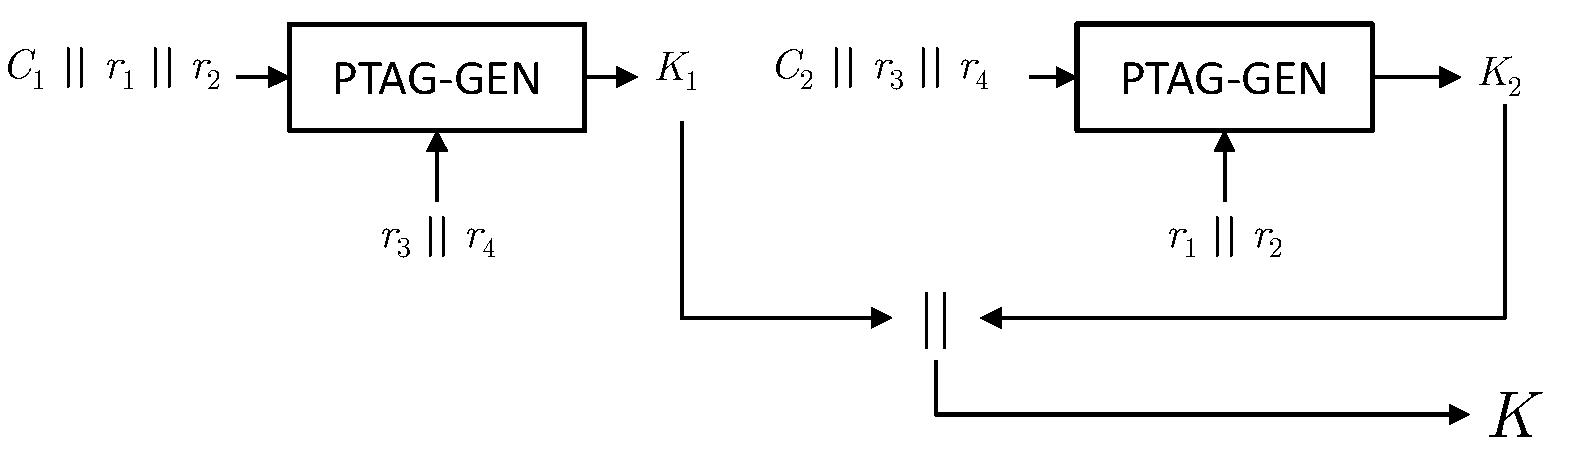
\includegraphics[width=0.7\textwidth]{key-construction}
% 	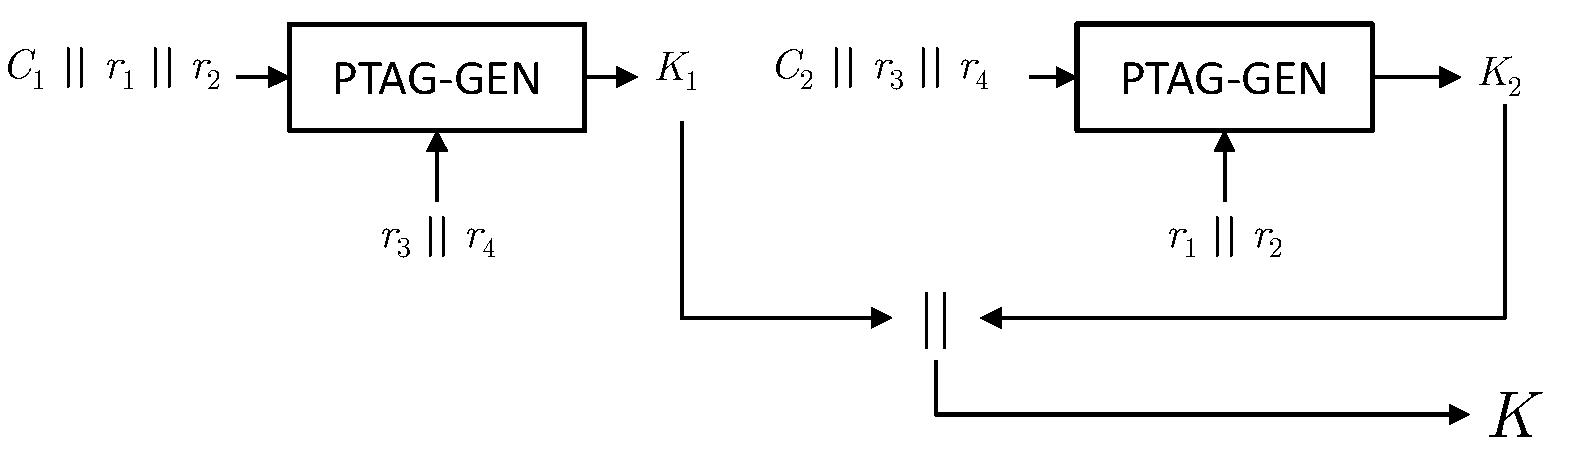
\includegraphics[scale=0.325]{key-construction}
	\caption{Key generation on \cshia.}
	\label{fig:key-construction}
\end{figure}

During the enrollment there were 8 challenges selected to produce four $r_i$ and four $w_i$ values. These challenges and helper data can be exposed off-chip and stored in \ptag~Memory if the designer chooses to do so. The recovery process of the secret key can be seen in \fregen. After using the challenges and all helper data, the syndromes are recovered. Due to inconsistent nature of \pufs, the fuzzy extractor actually recovers bit-flipped versions $w'_i$ and $r'_i$, what leads to the \bch~decoder receive $r'$ and $s'$. Once bit flips in $r_i$ values are corrected, the \fe~uses all $r_i$ to regenerate the secret key as Figure \ref{fig:key-construction} shows.

\subsection{Enrollment Phase}
\label{subsec:Enrollment-Phase}

In order to ensure authenticity and integrity, an initial procedure has to be conducted by the manufacturer\slash{}vendor. This enrollment procedure will activate the \fuzzy~to extract the secret key from \pufs. Once that is done, the \handler~brings all memory blocks for tag generation. Next, we detail this procedure.

\subsubsection{Key Extraction}
\label{subsubsec:Key-Extraction}

\ptag~Generator implements a Pseudo-Random Function (\prf), which is a primitive cryptographic very similar to a hash function with an important difference: the input processing is based on a secret key. In order to provide uniqueness to every \cshia~instance this key has to be unique. As aforementioned, \pufs~cannot be cloned, thus they can provide this uniqueness. Nevertheless, one big conundrum of using electronic \pufs~to generate keys is that they are inherently unstable. Due to their nature of leveraging on imperfection of the fabrication process, external factors such as temperature variation, voltage variation, etc., can interfere on their responses. Thus, varying responses to challenges during the lifetime of devices. In order to provide consistence in \puf~responses, \fuzzy~(\fe) are employed. In simple terms, \fes~are schemes comprised of an extraction algorithm and a recovery procedure. Becker provides a solid review and formal definitions in \cite{Becker2017:RobustFuzzyExtractor}.

There are multiple ways of implementing a \fuzzy. Originally, \cshia~was proposed using a Code-offset \fe, which is well-known to reduce entropy of extracted keys \cite{Armknecht2011:Formalization}. To strengthen the \cshia~design, we now use an adapted version of the Index-based Syndrome (\ibs) \fe~proposed by Yu and Devadas in \cite{Yu2010:RobustErrorCorrection}. \fenroll~illustrates the process of key extraction of \cshia's \fe. In general terms, a bit string $r$ is extracted from \pufs. Then, the \fe~generates a syndrome $s$ of $r$ using a $(n,k,t)$ Error Correction Code (\ecc). The \fe~also extracts a bit string $w$ and combines it to the syndrome $s$ to generate an encoded helper data $h$. This helper data $h$ can be externally exposed and will not leak information about $r$ (that can be used as secret key or derive the key).


\begin{figure*}[!ht]
	\center
	\subfloat[\fuzzy~during key extraction.]
	{
		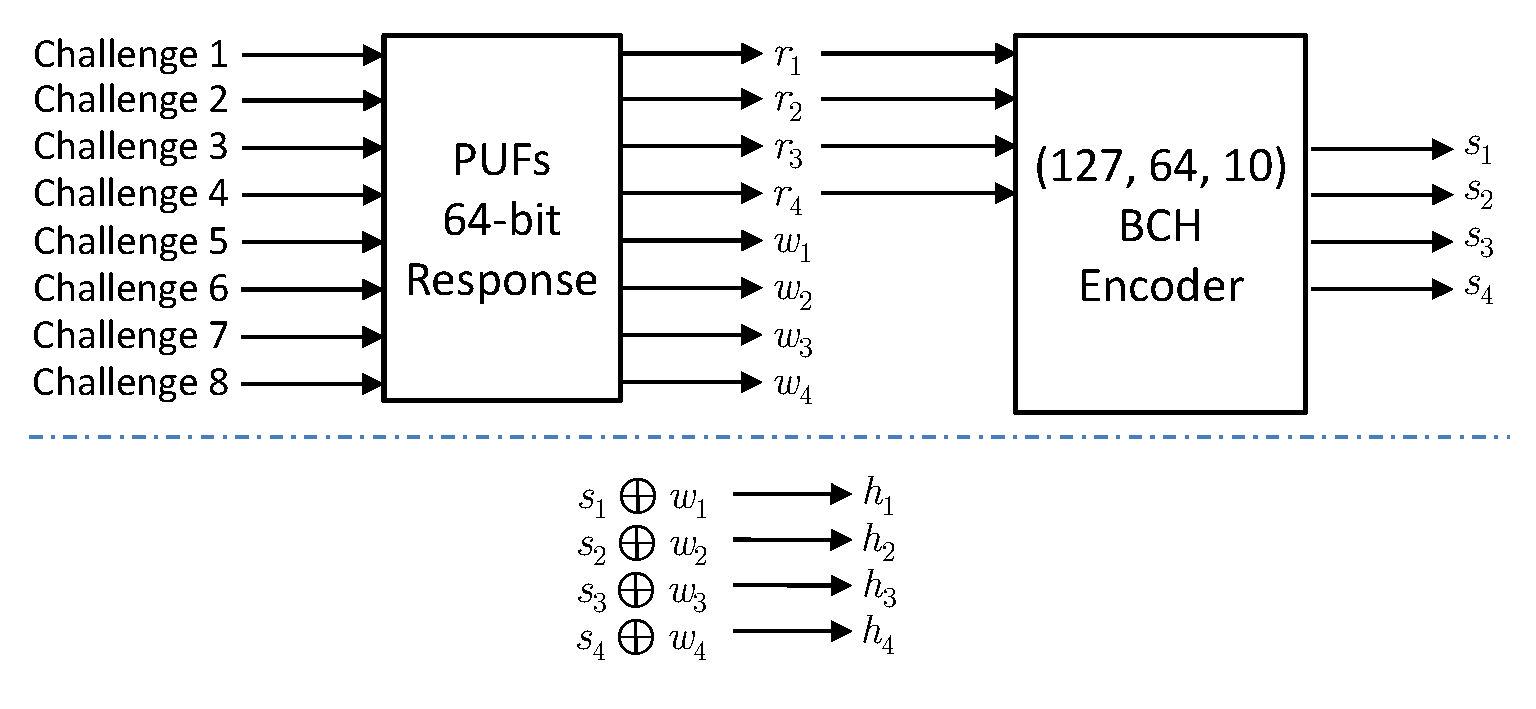
\includegraphics[scale=0.35]{fuzzy-enroll}
		\label{fig:fuzzy-enroll}	
	}
%	\hspace{0.1in}		
	\subfloat[\fuzzy~during key regeneration.]
	{
		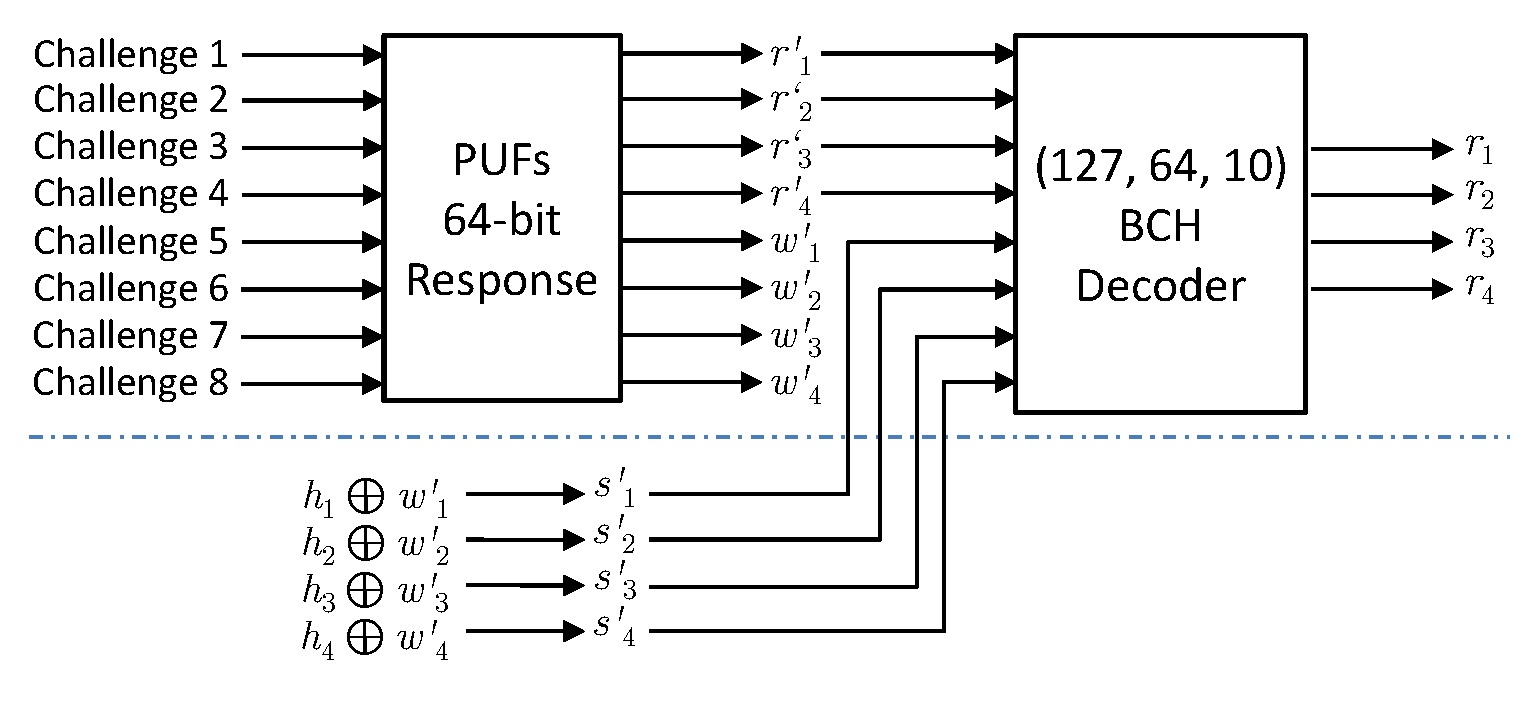
\includegraphics[scale=0.35]{fuzzy-regen}
		\label{fig:fuzzy-regen}
	}
%	\vspace{1in}		
%	\hspace{0.2in}		
	\caption{\fuzzy~actions during the enrollment and recovery procedure.}
%	\vspace*{-9pt} 
	\label{fig:fuzzy-extractor}
\end{figure*}


To fully explain \fenroll, the chosen parameters are detailed. First, \cshia~incorporates \pufs~that produce 64-bit responses (more details in the next section). These \pufs~will be responsible to generate each string $r$ and $w$ that are 64 bits long. To match the length of $r$ and $w$, \cshia~has a $(127, 64, 10)$-\bch~\ecc. As \fenroll~depicts, there are four bit strings $r_i$, which are compounded two by two and fed to the \prf~(Figure \ref{fig:key-construction}). Such combinations were specifically designed to match the \prf~chosen for \cshia, the \siphash~\cite{Aumasson2012:SipHash}, which has an output of 64 bits and uses key of 128 bits. Therefore, the first pair of bit strings $r_i$ is concatenated with a constant and processed by the \prf~using the second pair of bit string $r_i$ as key. That generates a hash $K_1$. Then, inverting their places and concatenating the second pair with a different constant, a hash $K_2$ is obtained. Concatenating $K_1$ with $K_2$ results in $K$ which is the secret key of \cshia. Notice that $C_1$ and $C_2$ in Figure \ref{fig:key-construction} are replacing addresses for input of the \ptaggen. Further details of security will be given in the following sections, however, one can notice that assuming that each bit string $r_i$ has at least half of their length of entropy, each part of the key will have full entropy. Hence, the key has full entropy. 

\subsubsection{Full Memory Protection}
\label{subsubsec:Full-Memory-Protection}

The Enrollment Phase proceeds to tag the memory range the manufacturer\slash{}vendor specified during design. Now that \ptaggen~has an unique key, \seceng~orders \handler~to bring all memory blocks and deliver them to it. \seceng~will use \ptaggen~to generate \ptags, however, depending on the solution against replay attacks a designer chooses, \ptaggen~is used differently. 

% \paragraph{Timestamps Generation}
% \label{paragraph:Timestamps-Generation}

% When timestamps are the solution against replay attacks, \pmmu~will have a timestamp memory. This timestamp memory has the depth of the number of data memory blocks the designer chose to cover. Thus, before \handler~hands in data memory blocks, \pmmu~will clear the entire timestamp memory to avoid uninitialized values. While \seceng~receives code memory blocks, generated \ptags~are just passed to \pmmu~that stores them in \ptagmem. As \handler~starts to pass data memory blocks to \seceng, \pmmu~increments the timestamp of each memory block received and passes this value to \seceng, which combines with the address of the memory block. This combination is then concatenated with the memory block and then finally hashed into a \ptag. \pmmu~receives this \ptag~and stores it in \ptagmem.

% \paragraph{\mt~Generation}
% \label{paragraph:Merkle-Tree-Generation}

% A \mt~solution is more complex. The first procedure is very straightforward. \seceng~receives memory blocks and their addresses from \handler~and uses \ptaggen~to generate \ptags. \pmmu~receives these \ptags~and sends them to \ptagmem. After all memory blocks had their \ptags~generated, \pmmu~starts to bring \ptags~of data memory blocks. As soon as a chunk of \ptags~is formed, a \ptag~internal address of the chunk is calculated. \pmmu~provides this internal address and the chunk to \ptaggen~that generates a \ptag. This \ptag~is returned to \pmmu~that stores it in \ptagmem. This process will continuously happen (as we can see in Figure \ref{fig:vtree}) until \pmmu~identify that the last \ptag~calculated has no siblings. Hence, it is the root \ptag, which must be stored inside \pmmu. It is worth to clarify that \ptag~internal address is an address space that facilitates computation and identification of descendants and ancestors. Each internal address is directly translated to a physical address by \pmmu~and this translation has as goal to minimize unused spaces in \ptagmem. Moreover, in terms of security, this internal address mitigates a very specific attack on the tree, in which an descendant has the same \ptag~as one of its ancestors. In this case, an attacker could try to perform a relocation attack likewise. 
